\newpage

\section{Dataset Description}

\quad For this project, we were provided with an excel file called "bebidas.xlsx", within which are the daily sales records of each of the two beverages made available by the company in question, within that excel file there are still other relevant data, which will be detailed afterwards. \\

In the following image we have a print of the columns of the dataset mentioned above:

\begin{figure}[H]
    \centering
    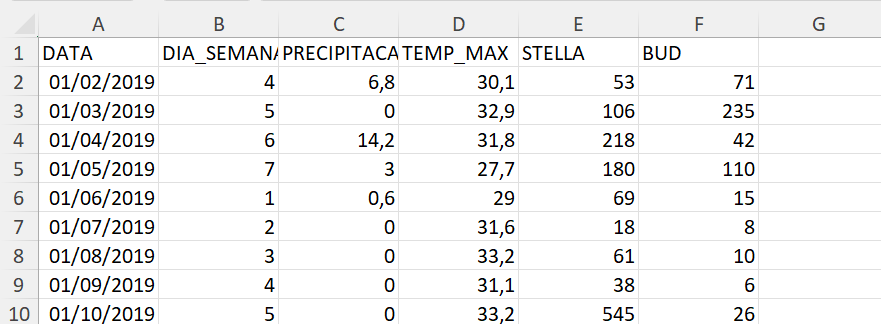
\includegraphics[width=0.8\textwidth]{assets/dataset.png}
    \caption{Project Dataset}
    \label{fig:dataset}
    \end{figure}


The following dataset is compose of 6 columns, they being:

\quad \textbullet DATA: This column represents the date the records are from;

\quad \textbullet DIA\_SEMANA: This column represents the day of the week, where 1 is Sunday, 2 is Monday, 3 is Tuesday, 4 is Wednesday, 5 is Thursday, 6 is Friday and 7 is Saturday;

\quad \textbullet PRECIPITACAO: This column represents the total of precipitation in mm in that day;

\quad \textbullet TEMP\_MAX: This column represents the daily maximum temperature in Celcius from that day;

\quad \textbullet STELLA: This column represents the number of STELLA drinks that where sold in that day;

\quad \textbullet BUD: This column represents the number of BUD drinks that where sold in that day.\\

To get a nice description of the values of each column we calculate the minimum value, the median, the mean, the max and other important values for each column, the next image represents the values that we got:\\

\begin{figure}[H]
    \centering
    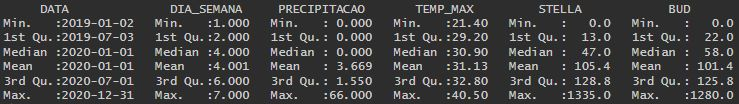
\includegraphics[width=0.8\textwidth]{assets/dataset-stats.jpeg}
    \caption{Dataset Statistics}
    \label{fig:dataset_stats}
    \end{figure}

These two diagrams represent the sales of each of the drinks provided in the dataset:
\\
\begin{figure}[H]
    \centering
    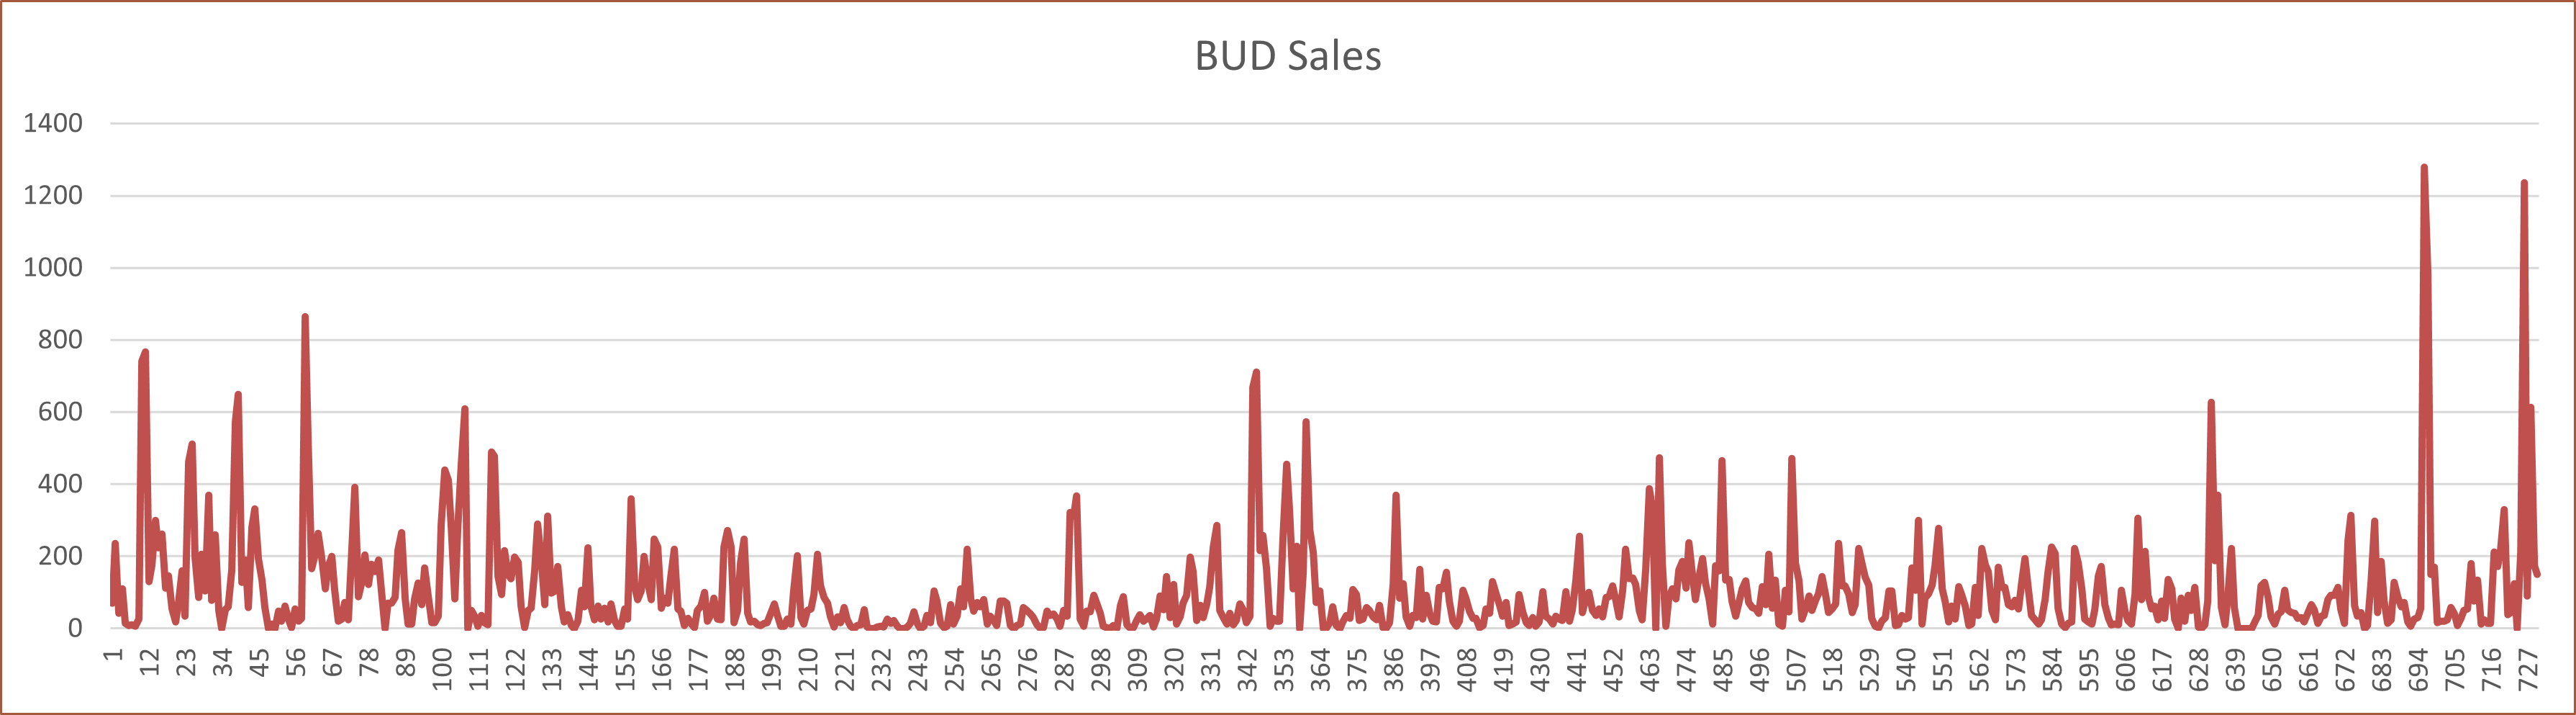
\includegraphics[width=0.8\textwidth]{assets/BUD.png}
    \caption{BUD Sales}
    \label{fig:bud_sales}
    \end{figure}

\begin{figure}[H]
    \centering
    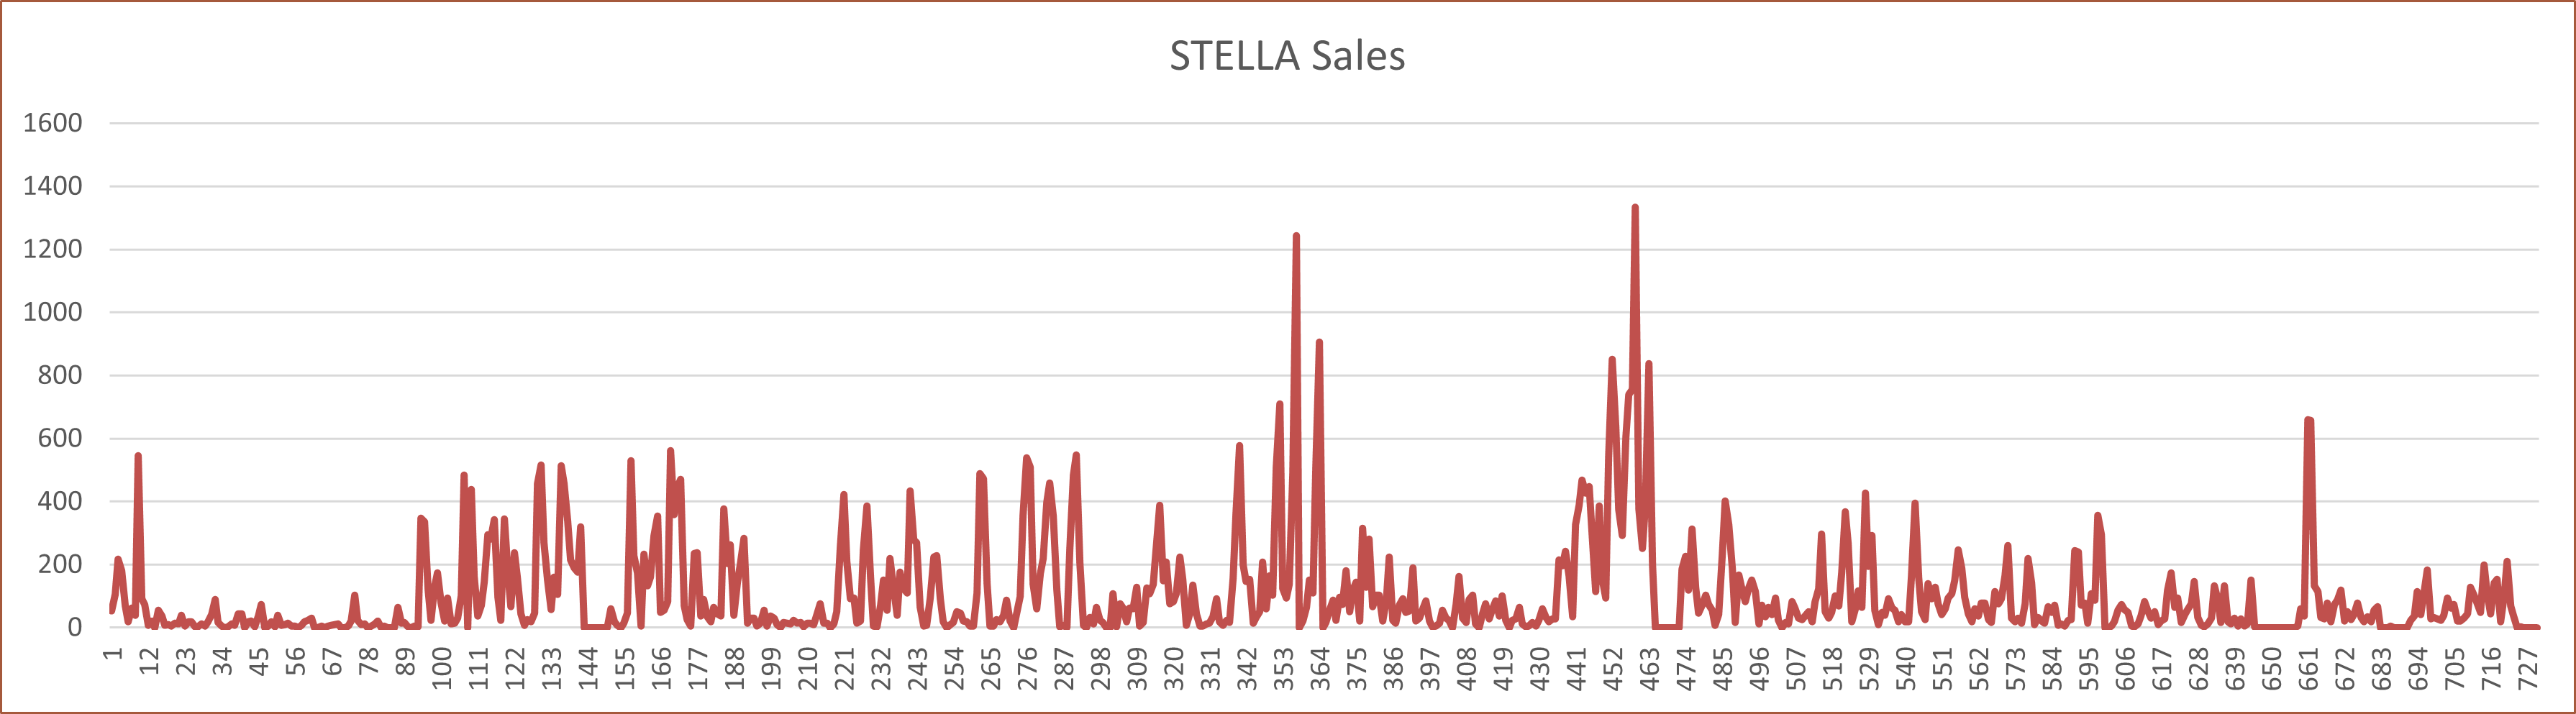
\includegraphics[width=0.8\textwidth]{assets/stella.png}
    \caption{STELLA Sales}
    \label{fig:stella_sales}
    \end{figure}

The next diagrams represent the outliers of sales data in realtion to the average sales of the respective dring (BUD and STELLA):\\

\begin{figure}[H]
    \centering
    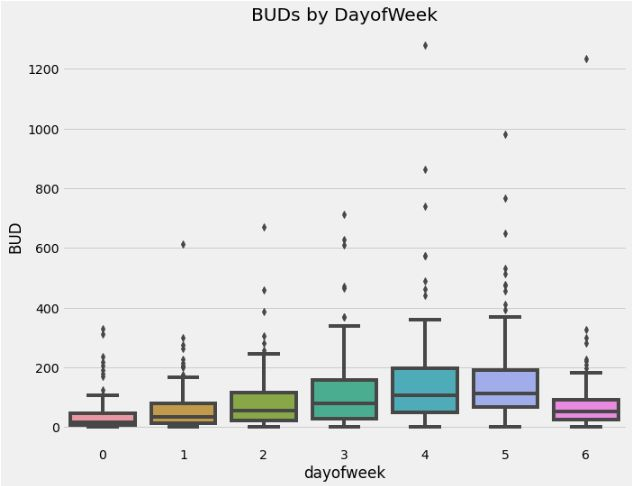
\includegraphics[width=0.4\textwidth]{assets/BUD-OUTLIERS.jpeg}
    \caption{BUD Outliers}
    \label{fig:bud_outliers}
    \end{figure}

    In this image we can see that int the BUD sales, there are more outliers in the Sunday and in Friday, but there are also some smaller outliers in the rest of the week, excluding Monday. \\


\begin{figure}[H]
    \centering
    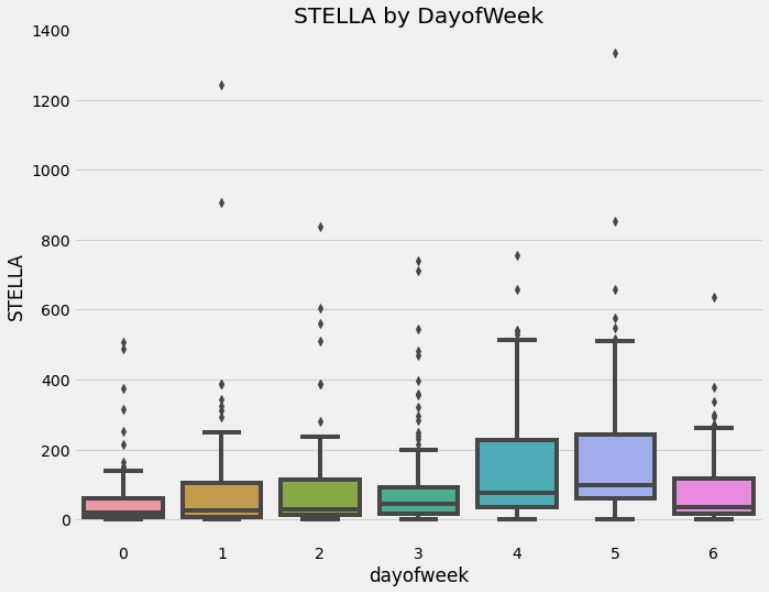
\includegraphics[width=0.4\textwidth]{assets/stella-outliers.jpeg}
    \caption{STELLA Outliers}
    \label{fig:stella_outliers}
    \end{figure}


In this image we can see that int the STELLA sales, there are more outliers in the Saturday and in Tuesday, but there are also some smaller outliers in the rest of the week, excluding Monday and Sunday. \\


The next two images will show the ACF of the STELLA sales and the BUD sales:


    \begin{figure}[H]
        \centering
        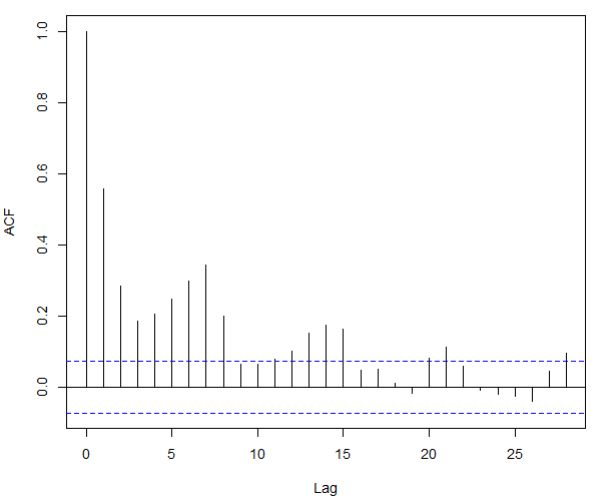
\includegraphics[width=0.6\textwidth]{assets/ACF STELLA.jpeg}
        \caption{ACF of STELLA}
        \label{fig:stella_outliers}
        \end{figure}


    \begin{figure}[H]
            \centering
            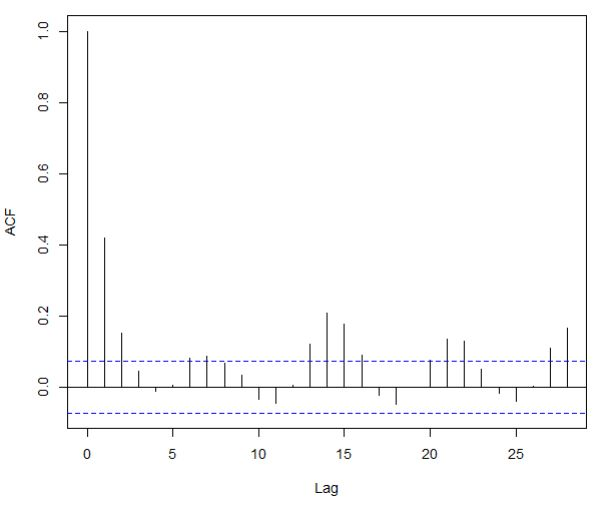
\includegraphics[width=0.6\textwidth]{assets/ACF BUD.jpeg}
            \caption{ACF of BUD}
            \label{fig:stella_outliers}
            \end{figure}



The next image will show the correlation of each one of the drinks with the rest of the columns values:\\

\begin{figure}[H]
    \centering
    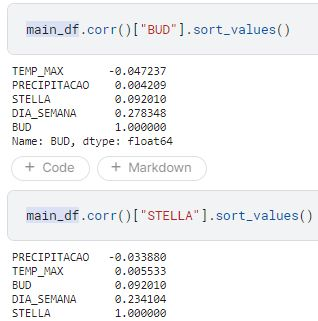
\includegraphics[width=0.6\textwidth]{assets/autocorrelação.jpeg}
    \caption{Correlation of STELLA and BUD}
    \label{fig:stella_outliers}
    \end{figure}
